\documentclass[border=0.9cm]{standalone}

% required packages and libraries
\usepackage{tikz}
\usetikzlibrary{automata, arrows.meta, positioning}

\begin{document}

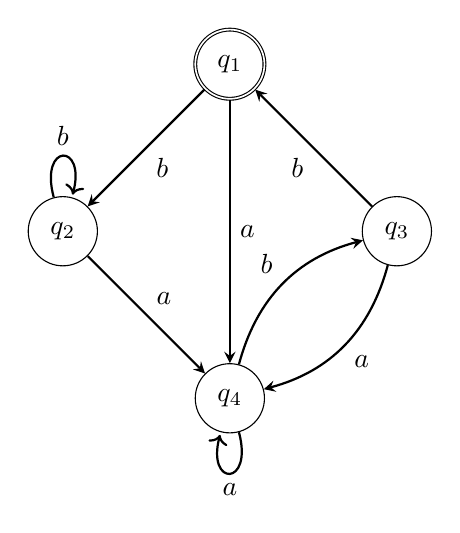
\begin{tikzpicture} [node distance = 3cm, on grid, auto]

\node (q2) [state] {$q_2$};
\node (q1) [state, accepting, above right = of q2] {$q_1$};
\node (q3) [state, below right = of q1] {$q_3$};
\node (q4) [state, below right = of q2] {$q_4$};

\path [-stealth, thick]
	(q1) edge node {$b$}   (q2)
	(q3) edge node {$b$}   (q1)
    (q2) edge node {$a$}   (q4)
    (q2) edge [loop above] node {$b$}   (q2)
    (q1) edge node {$a$}   (q4)
    (q4) edge [loop below] node {$a$}   (q4)
    (q4) edge[bend left] node {$b$}   (q3)
    (q3) edge[bend left] node {$a$}   (q4);
	% (c) edge [loop above]  node {$b$}()
	% (b) edge [loop below]  node {$b$}()
	% (b) edge[bend left] node {$b$} (d)
 %    (d) edge[bend left] node {$a$} (b)
 %    (e) edge node {$b$} (c)
 %    (e) edge node {$a$} (b)
 %    (d) edge node {$b$} (e);
\end{tikzpicture}

\end{document}
